\documentclass[11pt,a4paper]{article}
\usepackage[T1]{fontenc}
\usepackage{lmodern}
\usepackage[spanish,es-nodecimaldot]{babel}
\usepackage[a4paper,margin=2.4cm]{geometry}
\usepackage{graphicx,booktabs,tabularx,array,caption}
\usepackage{csquotes}
\usepackage[backend=biber,style=ieee,sorting=none]{biblatex}
\usepackage[hidelinks]{hyperref}
\Urlmuskip=0mu plus 1mu
\addbibresource{Referencias/referencias.bib}
\captionsetup{hypcap=false}
\setlength{\parskip}{0.45em}
\setlength{\parindent}{0pt}
\raggedbottom
\newcolumntype{Y}{>{\raggedright\arraybackslash}X}

\newcommand{\evidencia}[3]{%
  \begin{center}
    \includegraphics[width=\linewidth,height=0.63\textheight,keepaspectratio]{#1}
    \captionof{figure}{#2}\label{#3}
  \end{center}}
\begin{document}
\hypersetup{pageanchor=false}

\begin{titlepage}
\centering

{\Large Universidad Técnica Estatal de Quevedo\par}

\vspace{0.6em}

Facultad de Ciencias de la Computación y Diseño Digital\\
Carrera de Software

\vfill

{\large Aplicaciones Distribuidas (ISR-701)\par}

\vspace{0.5em}

{\large TA-IND-01 --- Informe Académico Individual\par}

\vspace{1.5em}

{\LARGE\bfseries
Análisis crítico de etcd\\[0.3em]
y comparación con Apache ZooKeeper\par}

\vfill

{\large Calderón Saltos Joseph Alexander\par}

\vspace{0.5em}

Paralelo: A\\
Fecha: 12 de noviembre de 2026


\vspace{2em}

{\small\bfseries Repositorio GitHub\par}

\vspace{0.5em}

\href{https://github.com/BelindaTZ/TA-IND-01-Informe-Acad-mico-Individual---CGMT/tree/main/Calderon\%20Joseph}{%
\resizebox{0.95\textwidth}{!}{%
\texttt{https://github.com/BelindaTZ/TA-IND-01-Informe-Acad-mico-Individual\mbox{-}\mbox{-}\mbox{-}CGMT/tree/main/Calderon\%20Joseph}%
}%
}
\par

\vfill

\end{titlepage}

\hypersetup{pageanchor=true}

\section*{Resumen}
etcd es un almacén distribuido de clave y valor que mantiene datos de configuración y coordinación, como el estado del plano de control de Kubernetes. Este informe examina cómo su API y el consenso Raft permiten acceder a un estado común desde distintos miembros. El análisis aplica las siete transparencias de distribución, CAP y PACELC, y contrasta el diseño de etcd con Apache ZooKeeper. En un clúster local de tres contenedores se escribió una clave, se consultó desde otro miembro y se detuvo el líder. Los dos miembros restantes eligieron un nuevo líder y confirmaron otra escritura. Tras reiniciar el miembro detenido, sus índices de Raft coincidieron con los del resto y la consulta desde ese nodo devolvió el valor escrito durante su ausencia. El resultado muestra que el clúster pudo reanudar las escrituras al conservar una mayoría. Un incidente documentado ilustra un límite de esa recuperación: índices de Raft iguales pueden coexistir con diferencias en los datos persistidos. La comparación sitúa la principal ventaja de etcd en sus lecturas linealizables por defecto y su coste en la coordinación necesaria para sostenerlas.

\section{Introducción}
Kubernetes necesita conservar un registro común de los recursos que administra y de sus cambios. Los componentes que consultan esa información deben poder trabajar sobre un estado coherente. Kubernetes usa etcd como almacén de los datos del clúster. El servidor de la API accede a ese almacén y los controladores operan a través de la API de Kubernetes \cite{kubernetes}. También pueden usar etcd directamente aplicaciones que necesiten guardar configuración o coordinar quién puede modificar un recurso \cite{etcdapi}.

La escala relevante tiene dos partes. En el laboratorio hay tres votantes y un único equipo físico. En un despliegue mayor, el número de trabajadores de Kubernetes puede crecer sin añadir un votante de etcd por trabajador. Cada votante conserva una copia del estado replicado y las escrituras dependen de una mayoría. Un grupo de cinco votantes puede soportar la pérdida de dos y necesita tres para confirmar cambios. Aumentar el grupo cambia tanto la tolerancia como el coste de coordinación \cite{etcdfaq}. Se eligió etcd porque permite observar esas consecuencias con un clúster local y comparar sus garantías con las de otro servicio de coordinación.

\section{Arquitectura del sistema}
La API v3 recibe solicitudes como \texttt{Put}, \texttt{Range} y \texttt{Txn}. Cada miembro dispone de un servidor, un componente Raft y almacenamiento persistente. Raft es el algoritmo de consenso que coordina la elección del líder y el orden de las operaciones en un registro. El almacén de claves aplica las entradas confirmadas y conserva revisiones para consultas y observación de cambios. El registro persistente permite recuperar el estado tras un reinicio \cite{etcdapi,etcdstorage}. Bora et al. formalizan en mCRL2 el comportamiento de Raft. Su trabajo permite distinguir el modelo de consenso del código que lo implementa \cite{bora2024raft}.

\evidencia{Anexos/Anexo_B_diagrama_etcd.pdf}{Diagrama del estudiante en draw.io. Los roles corresponden a un estado posible del clúster.}{fig:arquitectura}

El boceto del Anexo~\ref{an:boceto} ya representa al cliente, tres miembros y el paso de una escritura por el líder. El diagrama digital hace explícitos los puertos, distingue el acceso del cliente del tráfico entre pares y muestra dónde interviene el quórum. Su rótulo inferior corresponde a la fase de diseño del esquema. La ejecución posterior se documenta en la sección~\ref{sec:experimento}. Los nombres con guion pertenecen al esquema y los nombres sin guion identifican los servicios de Compose.

El cliente puede iniciar una escritura a través de un seguidor. El miembro receptor propone el cambio y el líder dirige la replicación. Con tres votantes, una escritura necesita la confirmación de al menos dos miembros. A esa mayoría se la conoce como quórum. El miembro receptor aplica el cambio confirmado antes de contestar. En nuestro experimento, los clientes se conectaron por el puerto interno 2379 y el tráfico entre miembros usó 2380. Solo \texttt{etcd1} publicó un puerto en el equipo anfitrión. Las pruebas usaron los nombres internos de los tres servicios.

\section{Análisis con los conceptos de la Unidad 1}
\subsection{Transparencias de distribución}
Las transparencias describen qué aspectos de la distribución quedan ocultos para quien utiliza el sistema \cite{vansteen2023}. En etcd su alcance depende de la operación y de la configuración del cliente \cite{etcdapi,etcdgar,etcdclient,etcdfail}.

\begin{description}
\item[Acceso.] La API ofrece la misma operación y representación de claves en los tres miembros. \texttt{etcdctl} usó el mismo \texttt{get} al consultar desde otro nodo.
\item[Ubicación.] El nombre de una clave no incluye el servidor que la almacena. La transparencia es parcial porque el cliente todavía necesita direcciones alcanzables para conectarse.
\item[Migración.] etcd conserva el espacio de claves al reemplazar un miembro mediante una reconfiguración. Mover el servicio o sus datos a otro clúster requiere intervención operativa y puede exigir cambiar los endpoints.
\item[Reubicación.] Un cambio de líder conserva el nombre de la clave y la API mientras el sistema está en uso. Una sesión conectada a un miembro que se apaga puede interrumpirse. etcd no traslada esa conexión activa al nuevo líder.
\item[Replicación.] El cliente envía una solicitud y Raft coordina las copias. El usuario no selecciona la réplica que debe guardar el cambio. Una lectura local serializable puede revelar retraso entre réplicas.
\item[Concurrencia.] Las escrituras confirmadas tienen un orden común. Una transacción puede comparar la revisión de una clave y escribir solo si coincide. La aplicación que hace una lectura seguida de una escritura independiente debe manejar por su cuenta el conflicto entre ambas.
\item[Fallos.] La elección y la puesta al día del miembro son automáticas ante un fallo temporal que conserve el quórum. Durante la elección o al perder el endpoint pueden aparecer errores y tiempos de espera.
\end{description}

\subsection{CAP y PACELC}
En CAP, la consistencia se entiende como una vista linealizable y la disponibilidad exige que cada solicitud a un nodo operativo pueda completarse, incluso durante una partición. En una división de dos miembros contra uno, el lado mayoritario puede elegir líder y confirmar escrituras. El lado aislado no puede confirmar una escritura ni sostener por sí solo la lectura linealizable. Por eso las operaciones fuertes de etcd se clasifican como CP. Una lectura local de un miembro aislado puede devolver una revisión anterior y ofrece otra garantía \cite{vansteen2023,etcdgar,etcdfail}.

PACELC examina además lo que ocurre con la red sana. Una escritura espera la replicación suficiente y una lectura linealizable requiere comprobar que el miembro tiene acceso al estado confirmado bajo un líder válido. En ambas rutas etcd prioriza consistencia, con coste de coordinación. La opción \texttt{serializable} permite responder con el estado local y prioriza la latencia de esa lectura a cambio de posible desfase. En PACELC, esto se resume como PC/EC: se mantiene la consistencia durante una partición y también se prioriza cuando la red funciona normalmente, aunque eso cueste tiempo de respuesta. Es una interpretación de las garantías de la API, no una medición de esta práctica. La prueba de este informe no midió latencia ni aisló la red \cite{etcdgar,vansteen2023}.

\subsection{Modelos de comunicación}
El diseño combina un modelo cliente-servidor en la API con comunicación entre pares dentro del clúster. Los pares pueden votar y cambiar de rol, aunque el líder dirige la replicación en cada término. El cliente de la API v3 usa llamadas gRPC sobre HTTP/2 y TCP. \texttt{Put} y \texttt{Range} siguen el patrón petición-respuesta. El cliente de línea de comandos espera la respuesta o el vencimiento de su plazo \cite{etcdapi,etcdclient}.

\texttt{Watch} mantiene un flujo de eventos desde revisiones de claves. El cliente puede recibir cambios sin sondear la clave en un bucle. Si se interrumpe el flujo, la revisión conocida sirve para reanudarlo mientras siga disponible en el historial. Entre servidores, los mensajes de Raft transportan votos, latidos y entradas de registro. Se envían a través de conexiones entre miembros. La confirmación de una escritura sigue dependiendo de la mayoría \cite{etcdapi,etcdgar,etcdfail}.

\subsection{Tolerancia a fallos e incidente documentado}
Con tres votantes se tolera la indisponibilidad de uno mientras los dos restantes puedan comunicarse. Cuando dejan de llegar latidos del líder y vence el tiempo de elección, un seguidor puede solicitar votos. Con una mayoría se elige otro líder. Al volver, el miembro rezagado puede recibir las entradas faltantes o una instantánea si el registro necesario ya no está disponible. Si se pierden permanentemente dos votantes, se requiere recuperación operativa. Un timeout de cliente deja incierto el resultado de la operación, por lo que repetir una actualización de estado puede requerir una comparación de revisión \cite{etcdfail,etcdgar,etcdrecovery}.

En marzo de 2022 se reportó un clúster de tres miembros en etcd 3.5.1 con índices Raft iguales y revisiones distintas. El equipo de etcd vinculó el reporte a un fallo de persistencia al caer un miembro bajo carga \cite{etcdissue}. El índice persistente podía avanzar antes de que se confirmaran los datos en el almacén. Una caída entre ambos pasos dejaba un índice que indicaba más progreso del que se había guardado. El problema se introdujo en v3.5.0 y se corrigió en v3.5.3 \cite{etcdincident}. El caso distingue el acuerdo sobre el registro de su aplicación durable en cada réplica.

Otro fallo puede manifestarse en el lado cliente. El diseño del cliente documenta reconexiones, selección de endpoints y plazos \cite{etcdclient}. Incluso con mayoría, una conexión interrumpida puede devolver un error antes de recuperar acceso. El ensayo local consultó explícitamente los dos endpoints activos después de detener al líder.

\section{Experimentación propia}\label{sec:experimento}
El registro del 12 de noviembre documenta tres contenedores de etcd 3.7.3 en Docker Desktop para Windows 11, cada uno con volumen persistente. El archivo \texttt{Experimento/compose.yaml} define los miembros. Al iniciar, Windows rechazó la publicación del puerto 12379. El registro describe cómo se retiró la publicación de \texttt{etcd2} y \texttt{etcd3} para usar su red interna. Los comandos completos y sus resultados están en \path{Experimento/comandos_y_resultados.md}. La tabla~\ref{tab:prueba} conserva los datos que permiten interpretar la secuencia.

\begin{table}[!ht]
\centering
\caption{Secuencia observada en el experimento}\label{tab:prueba}
\begin{tabularx}{\linewidth}{@{}p{0.26\linewidth}YY@{}}
\toprule
Paso & Operación & Salida observada \\
\midrule
Inicio (fig.~\ref{fig:estado}) & \texttt{endpoint status -w table}, tres endpoints & Líder \texttt{etcd3}, término 3, índices 11/11. \\
Escritura y lectura (fig.~\ref{fig:lectura}) & \texttt{put} por \texttt{etcd1}, \texttt{get} por \texttt{etcd2} & \texttt{OK} y \texttt{Replicacion-etcd}. \\
Caída (fig.~\ref{fig:caida}) & \texttt{docker compose stop etcd3}, consulta de dos endpoints & Líder \texttt{etcd1}, término 4, índices 14/14. \\
Escritura con dos miembros (fig.~\ref{fig:quorum}) & \texttt{put} por \texttt{etcd2}, \texttt{get} por \texttt{etcd1} & \texttt{OK} y \texttt{quorum-2-de-3}. \\
Recuperación (fig.~\ref{fig:regreso}) & \texttt{docker compose start etcd3}, estado y \texttt{get} por \texttt{etcd3} & Líder \texttt{etcd1}, término 4, índices 16/16 y valor \texttt{quorum-2-de-3}. \\
\bottomrule
\end{tabularx}
\end{table}

El cambio del término 3 al 4 y el reemplazo de \texttt{etcd3} por \texttt{etcd1} son evidencia de una elección. El segundo \texttt{OK}, seguido de una lectura por otro endpoint, muestra que la mayoría confirmó un dato nuevo con el líder inicial detenido. Tras el reinicio, los índices aplicados iguales aportan evidencia de que el miembro reincorporado alcanzó la posición observada en los demás. La lectura desde ese endpoint comprueba que podía servir el valor creado durante su ausencia.

El primer intercambio muestra acceso uniforme y una vista común de la clave. La segunda escritura comprueba progreso con quórum tras una elección. Las capturas son observaciones puntuales. El intervalo entre ellas incluye tiempo de intervención manual y no sirve para estimar la duración de la elección. \texttt{docker compose stop} provoca una detención controlada. Los tres procesos comparten equipo y red virtual. El ensayo cubre la pérdida de un proceso y su retorno, con alcance distinto al de una partición, una pérdida de disco o un fallo del anfitrión.
\section{Ejemplos del entorno del estudiante}

\subsection{Sistema de Gestión Académica de la UTEQ}

En el SGA de la UTEQ subo tareas y consulto las actividades de mis asignaturas. Después de realizar una entrega, reviso su estado para comprobar que haya quedado registrada. Aunque acceda nuevamente a la plataforma, espero encontrar la información que guardé anteriormente.

Esta situación se relaciona con la transparencia de acceso y la consistencia de los datos. Como estudiante, me interesa que la entrega quede registrada y pueda consultarla después, sin tener que conocer los servidores que utiliza la plataforma. Sin embargo, esta experiencia no permite determinar cómo almacena o replica la información el SGA.

\subsection{WhatsApp}

En WhatsApp puedo enviar un mensaje y observar sus estados de envío, entrega y lectura. Estos indicadores no siempre cambian al mismo tiempo, ya que dependen de las condiciones de comunicación y de la disponibilidad del destinatario.

Lo relaciono con la comunicación asíncrona en los sistemas distribuidos. El emisor y el receptor no necesitan estar interactuando al mismo tiempo para intercambiar mensajes. Los indicadores permiten conocer parte del estado de la comunicación, aunque no muestran cómo se procesa internamente cada mensaje.

\section{Análisis comparativo con Apache ZooKeeper}
La comparación toma las garantías de etcd y las documentadas por Apache ZooKeeper \cite{etcdapi,etcdgar,etcdfail,zookeeper,zkadmin}.

\begin{table}[!ht]
\centering
\caption{Comparación técnica de etcd y Apache ZooKeeper}
\begin{tabularx}{\linewidth}{@{}p{0.20\linewidth}YY@{}}
\toprule
Criterio & etcd & Apache ZooKeeper \\
\midrule
Acceso y datos & Claves en un espacio plano, con rangos por prefijo y revisiones. & Árbol de znodes con rutas y versiones. \\
Consenso y escritura & Raft replica el registro y confirma con mayoría. & Zab, su protocolo de difusión, ordena los cambios desde el líder y necesita quórum. \\
CAP y partición & El lado sin mayoría no puede avanzar operaciones fuertes. & El lado sin quórum no confirma escrituras. El modo opcional de solo lectura puede servir datos locales. \\
Latencia y consistencia & Lectura linealizable por defecto. Lectura local serializable opcional. & Las lecturas ordinarias se sirven desde el servidor conectado y pueden ir retrasadas. \\
Comunicación & RPC gRPC y flujo \texttt{Watch} por revisiones. & Protocolo cliente-servidor sobre TCP y avisos de cambios. Los watches clásicos se disparan una vez. \\
Concurrencia & \texttt{Txn} compara versiones, revisiones o valores. & Actualizaciones condicionadas a una versión y operaciones agrupadas con \texttt{multi}. \\
Fallos y sesión & Reelección, reconexión del cliente y claves asociadas a \textit{leases}. & Reelección, reconexión dentro del plazo de sesión y znodes efímeros ligados a la sesión. \\
\bottomrule
\end{tabularx}
\end{table}

El punto de decisión es qué debe saber la aplicación al leer. Si un controlador actúa sobre la última configuración confirmada, la lectura linealizable por defecto de etcd encaja con esa necesidad. Si el servicio se organiza alrededor de rutas jerárquicas, sesiones y presencia representada por znodes efímeros, ZooKeeper ofrece esas abstracciones directamente. Su lectura local ordinaria es atractiva para consultas que admiten atraso. En una decisión que dependa del dato más reciente, ese atraso debe tratarse explícitamente. La comparación describe el diseño y las garantías. El laboratorio usó solo etcd.

\section{Postura crítica}
La ventaja de etcd es que la mayoría y las revisiones ofrecen una base clara para coordinar cambios. En el laboratorio, cambiar de líder y mantener dos miembros bastó para volver a escribir. El coste aparece cuando las escrituras cruzan enlaces lentos o los discos demoran la persistencia. En esos casos, añadir réplicas puede aumentar el coste operativo y no reparte automáticamente el trabajo del líder \cite{etcdfaq}. Du et al. proponen otra estrategia de elección y Shang et al. estudian una organización de Raft en dos niveles. Yu et al. proponen adaptaciones para redes inalámbricas \cite{du2023leader,shang2025draft,yu2024adaptive}. Son propuestas de investigación y sus resultados corresponden a sus propios escenarios.

Usaría etcd para configuración y coordinación donde una lectura atrasada pueda causar acciones incompatibles. Para guardar telemetría de alto volumen o para aplicaciones que deban seguir escribiendo en ambos lados de una partición, sus garantías y la dependencia del quórum encajan peor \cite{etcdfaq,etcdgar}. La decisión depende de qué operaciones toleran atraso y cuáles requieren conocer el último estado confirmado.

Un ensayo de caída y retorno comprueba un recorrido concreto. Gulcan et al. usan modelos para guiar la exploración de estados en implementaciones distribuidas, incluida Etcd-raft \cite{gulcan2025modelfuzz}. Borgarelli et al. emplean recompensas de exploración para dirigir las pruebas hacia escenarios difíciles de alcanzar \cite{borgarelli2024reward}. Los dos trabajos explican por qué una elección exitosa en una práctica local deja abiertas preguntas sobre fallos combinados y secuencias de mensajes.

\section{Conclusiones}
\begin{enumerate}
\item La caída del líder inicial cambió el término de 3 a 4. Con dos votantes activos, etcd confirmó una nueva escritura y la lectura por otro miembro devolvió el valor esperado.
\item Al reincorporarse \texttt{etcd3}, los tres miembros mostraron índice aplicado 16 y el endpoint recuperado sirvió el valor escrito durante el fallo. La igualdad de índices y la lectura sostienen la puesta al día observada.
\item La comparación con ZooKeeper distingue dos rutas de lectura. etcd ofrece linealizabilidad por defecto y ZooKeeper sirve lecturas ordinarias desde el miembro conectado. La elección afecta qué tan reciente debe ser la información para que la aplicación actúe correctamente.
\end{enumerate}

\section*{Declaración de uso de inteligencia artificial}
Se utilizó ChatGPT (GPT-6) y ChatGPT Work como apoyo para organizar el informe, preparar borradores en LaTeX, revisar referencias bibliográficas y consultar documentación técnica. La herramienta también ayudó a seleccionar y resaltar fragmentos de tres artículos académicos.

El experimento con etcd se ejecutó en un entorno local con Docker. Los comandos, sus resultados y las capturas originales quedaron registrados en el repositorio. Las fuentes consultadas se contrastaron con sus publicaciones y enlaces oficiales. La revisión final del contenido y la explicación de los resultados corresponden al estudiante.

\clearpage
\printbibliography[title={Referencias}]

\clearpage
\appendix
\section{Bosquejo de arquitectura a mano}\label{an:boceto}
\begin{center}
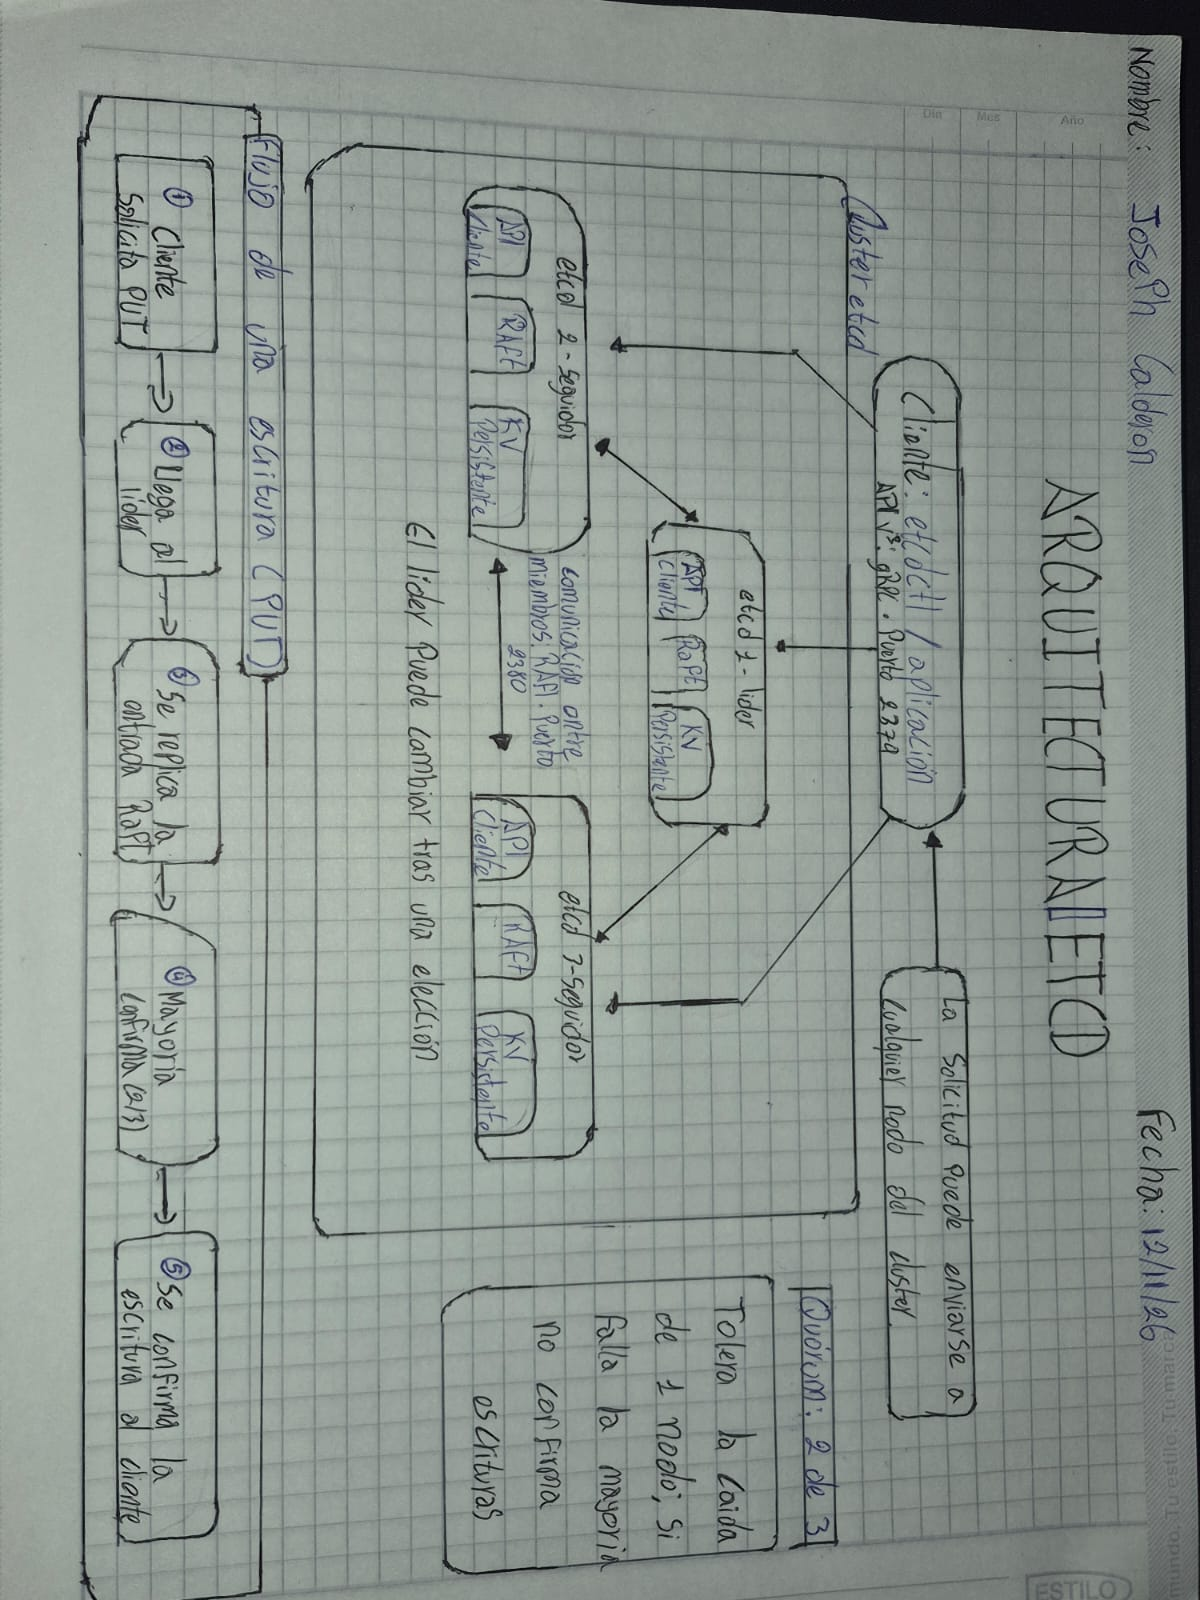
\includegraphics[width=\linewidth,height=0.78\textheight,keepaspectratio]{Anexos/Anexo_A_bosquejo_etcd.jpg}
\end{center}

\clearpage
\section{Capturas de lectura de fuentes}
Las páginas provienen de versiones publicadas. 
Las capturas corresponden a tres artículos citados en el informe.
Se incluyen los fragmentos utilizados y sus páginas
para relacionarlos con el análisis técnico.

\evidencia{Anexos/lectura_bora.png}{Bora et al., p.~8. Elección y replicación en el modelo de Raft \cite{bora2024raft}.}{fig:bora}
\clearpage
\evidencia{Anexos/lectura_gulcan.png}{Gulcan et al., p.~282:2. Uso de un modelo abstracto para medir cobertura \cite{gulcan2025modelfuzz}.}{fig:gulcan}
\clearpage
\evidencia{Anexos/lectura_borgarelli.png}{Borgarelli et al., p.~339:3. Recompensa para explorar estados nuevos \cite{borgarelli2024reward}.}{fig:borgarelli}

\clearpage
\section{Capturas del experimento}
\evidencia{Experimento/Capturas/01_estado_cluster.png}{Estado inicial de los tres miembros.}{fig:estado}
\clearpage
\evidencia{Experimento/Capturas/02_escritura_lectura.png}{Escritura por etcd1 y lectura por etcd2.}{fig:lectura}
\clearpage
\evidencia{Experimento/Capturas/03_caida_lider.png}{Estado posterior a la detención de etcd3.}{fig:caida}
\clearpage
\evidencia{Experimento/Capturas/04_escritura_durante_fallo.png}{Confirmación y lectura con dos miembros activos.}{fig:quorum}
\clearpage
\evidencia{Experimento/Capturas/05_recuperacion_nodo.png}{Estado de los tres miembros y lectura desde etcd3 tras el reinicio.}{fig:regreso}
\end{document}



